\chapter{Mobile User Experience}

\section{Aims}
\paragraph{} At the end of this topic you will be able to:

\begin{itemize}
\item Use design patterns to communicate your designs
\item Use and understand platform guidelines
\item Evaluate your application
\end{itemize}

\paragraph{} Whilst there are many core lessons to be learnt from human factors research about the best ways to design software for different users which are generally applicable, it is also true that the mobile platform offers some aspects of the user experience which are particular to the mobile context. For example, the close integration of a wide array of physical sensors, human and machine oriented communication support, wide-variety of screen sizes, touch interface, lack of hardware keyboard, wireless/untethered operation, and pure ubiquitousness provide both unique opportunities to take advantage of and novel pitfalls to avoid.


\section{Design Patterns}
\paragraph{} Design patterns can be considered as an attempt to build a shared language for describing solutions to problems. They were originated in the architectural research discipline by Christopher Alexander who coined the term ``Pattern Language''. An individual pattern describes a problem, and a solution. Importantly, patterns were originally specified as `timeless' e.g. they didn't make assumptions about the adoption of a particular technology or intricate solution to a one-off issue, but were more about dealing with recurring problems that have accepted and acknowledged solutions that are both beautiful and practical. A key element of patterns is the idea of language. A collection of design patterns forms a shared language for communicating ideas about recognising and solving problems. By having a shared language people, any people, not just experts, can understand and contribute towards the solution of the problem.

\subsection{Patterns as a Dictionary of Decisions}
\paragraph{} One nice way to describe patterns is as entries in a dictionary. When a designer creates a design they make decisions about how to solve problems. Often these problems and solutions recur many times in many contexts. A pattern is thus a single, documented problem and its most common, recognised, good solution. Each pattern is named, described, and cross-referenced to related patterns similar to entries in a dictionary. In this way the collection of patterns form a language, having syntax, the description of individual patterns, grammar and semantics, captured by the relations between patterns.

\paragraph{} The idea of pattern languages was borrowed by Software Engineers in the 1990s who started applying the idea of recurring and reusable solutions to the design and development of computer software.

\paragraph{} The Android platform, like software design in general\footnote{The Portland Pattern Repository found at \url{http://c2.com/cgi/wiki?WelcomeVisitors} is probably the best online resource about software design patterns. Interestingly it was also one of the first Wikis on the web. Of course the best `dead tree' edition is the `gang of four book' \cite{gamma_1994_design.patterns}. However this book is aimed at experience software engineers so a better place to start might be the `Head First Design Patterns' book \cite{freeman_2004_head.first.design.patterns}} has it's own sets of design patterns\footnote{\url{https://developer.android.com/design/patterns/index.html}} related to patterns of interaction with Android user interface elements.

%\section{Design Patterns for Mobile \& Android}


\section{Style Guides}
\paragraph{} Recently, the Android project has developed Material Design\footnote{\url{https://developer.android.com/design/material/index.html}}, a guide for visual, motion, and interaction design across platforms and devices. Similarly Apple has had the iOS Human Inteface Guidelines \footnote{\url{https://developer.apple.com/library/ios/documentation/UserExperience/Conceptual/MobileHIG/}} for many years. The aim of these guide is twofold. Firstly, to build on the same ideas as design patterns by giving everyone an agreed language for sharing and communicating aspects of our designs. Secondly, style guides define a baseline for designing software for their respective platforms. If the guides are followed this leads to greater cohesion of apps across the platform which shows respect for users by matching their expectations. Of course, the recent popularity of touch interfaces and design to suit the vagaries of differing mobile platforms means that most of these style guides are in flux. They are living documents which are regularly updated to try to capture best practise as we learn and discover new and better ways to build and use mobile apps.


\section{Evaluation}
\paragraph{} You should not leave evaluation of your app until the very last moment as it is then far too late to fix any basic errors in usability or misunderstandings of your target users. So you should evaluate early and often. For now, we will assume that we are evaluating a prototype at some stage of its development from basic layout with little functionality (lo-fi – low fidelity) to almost the final product (hi-fi prototype).

When you have conducted your evaluation, made any changes, re-tested - you’re good to go - deploy \& market (something we will look into towards the end of the module).

\subsection{Evaluation Techniques}

\begin{quote}
``Evaluation is about humility'' Jones \& Marsden
\end{quote}

\paragraph{} Leave your ego outside the usability lab and hope it won't be an exercise in complete humiliation. Here are a few techniques presented in order from basic lo-fi prototype being required up to techniques for evaluating a near-finished product :

\subsubsection{Quick feedback}
\paragraph{} Completely unscientific, but useful for some informal feedback on a lo-fi prototype – simply get a few typical end-users together and show them your work. Take notes. Use this to check your ideas aren’t miles out.

\subsubsection{Conceptual Model Extraction}
\paragraph{} Use storyboard sketches or a lo-fi model to show to users. Ask them to explain what they think you are trying to convey. For example, look at the Android emulator or phone homepage. Should settings be a couple of cogs? The users should be able to extract your conceptual model from your prototype/ sketches.

\subsubsection{Direct Observation}
\paragraph{} Give users some instructions and your prototype and observe how well they manage to undertake your tasks. You might ask them to think aloud and record their thoughts on a Dictaphone (or your phone) or you could video the session so you can observe without taking notes and reply later. You can use a log to capture the users' interactions – use the logging feature of Android to provide a trace of where the user went in your app and how long they stayed there. Heat maps are also interesting but they are not yet commonplace for mobile devices:

\begin{figure}[H]
\centering
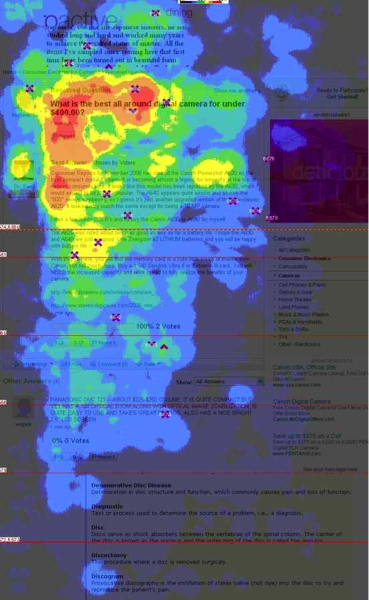
\includegraphics[width=0.75\textwidth]{images/heatmap}
\caption{Heatmap used to visualize where a users eyes spend their time}
\label{fig:heatmap}
\end{figure}

\paragraph{} In any evaluation, even if it’s for your coursework, look after your users:
\begin{itemize}
\item Follow any ethics guidelines eg don’t expose children to inappropriate material or excessive volume etc
\item Explain what you want and why
\item Treat them with respect – e.g. don’t roll your eyes if they get it all wrong
\item Let them withdraw if they have had enough
\item Reward them – be prepared to pay them – or if it’s a coursework reciprocate
\end{itemize}

\subsubsection{Interviews}

\paragraph{} Rather than just observing users - ask them what they think, why they approached tasks in the way they did etc. This can follow on from observation or, if you can’t observe for some reason, can be used as a substitute.

\subsubsection{Questionnaires}
\paragraph{} Everyone loves a good questionnaire. I know - you hate them - but for the developer they are easy and can reach a wide audience. The questionnaire returns can usually be analysed quantitatively (eg ``30\% got to the app icon first go'', ``18\% agreed that the text was easy to read''). Don’t just throw together some questions in five minutes - you only get one chance - study the theory of questionnaire design. It’s easy to make a mess of it and then you have lost your opportunity to gain valuable feedback.

\paragraph{} The following are some guidelines for good practice in questionnaire design:
\begin{itemize}
\item The complexity of your questionnaire and its language should take into account the age, education, competence, culture, and language abilities of respondents.
\item Consider using:
\item E-mail – fast, inexpensive, not anonymous.
\item Telephone – time consuming, not anonymous, may require skill, has to be short.
\item Face-to-face interview – slow, expensive, requires skill, best for small samples, qualitative studies.
\item Web-based – fast, inexpensive, can be anonymous, best for large surveys, for example use http://www.surveymonkey.com
\item Explain the purpose of the work – emphasise that it’s a worthwhile use of their time and they are contributing to something worthwhile and their feedback is important. Thank them too.
\item Keep it short and let them know how long it’ll take.
\item Use a good structure – group questions into sections. Let them skip or backtrack.
\item Keep response options simple, for example, use scales that provide useable granularity or consider a Lickert scale\footnote{\url{http://en.wikipedia.org/wiki/Likert_scale}}.
\item Be consistent don’t use a 5-point scale in one question and a 7-point in the next.
\item If you use a continuum scale with numbers for answer options, use a clear concept at the top and bottom of the scale (eg “on a scale of 1 to 5, how good is it? : where 1=very bad and 5=very good).
\item Use scales that are centred– don’t have one “bad” answer option and four shades of “good”.
\item Don’t force respondents into either/or answers if a neutral position is possible
\item ``Not applicable'' or ``don’t know'' responses should be available
\item Open responses are difficult for you to consolidate, so use them sparingly – but they can sometimes provide the best information, eg “what would you change?” but don’t force them to answer.
\end{itemize}

\subsubsection{Usability experts}
\paragraph{} Employ a trained usability expert and draw on their training and expertise. They would be considering the following heuristics (ie applying their experience gained/ knowledge to a problem) (Jones \& Marsden, 2006):

\begin{itemize}
\item Visibility of system status – does the user know where he is, what’s going on
\item Match between system and real-world – is the language right
\item User control and freedom – support undo/redo to help users who make mistakes
\item Consistency and standards – follow Android/ iPhone conventions
\item Error prevention – better to prevent than report errors eg restrict input
\item Flexibility and efficiency – responsiveness for users, let them tailor frequent actions
\item Aesthetic/ minimalist design – don’t overdo prompts etc
\item Recovery – help users recover if stuck or make a mistake
\item Help \& documentation – timely, appropriate help
\end{itemize}

\subsubsection{Experimental Evaluation}
\paragraph{} Here we try to evaluate our app with something similar. For example, compare Android  with iPhone. We pick one metric eg user errors and conduct a series of experiments such as asking the user to open a browser and find a site. You then use statistical analysis on recorded keypresses/ clicks to determine if the users were more likely to make an error using iPhone than Android then how long they took to overcome the error. 

\paragraph{} How do you know if the data is right about which would cause the fewest errors?  The skill is in the design of the experiment and the analysis tools used.

\subsection{Case Studies}
\subsubsection{Smart Diet}

\paragraph{} A group of researchers from Seoul, Korea developed a SmartDiet app then setup an experiment with 19 overweight people who used the app and a further 17 people who were asked to lose weight without the app\footnote{\url{http://jtt.rsmjournals.com/cgi/content/abstract/16/5/270}}. Overall, the researchers found that ``the SmartDiet mobile weight management application appears to contribute to weight loss in obese adults''.

\begin{figure}[H]
\centering

\includegraphics[width=0.5\textwidth]{images/smart-diet-1}
\caption{Smart Diet Launch Screen}
\label{fig:smart-diet-1}
\end{figure}

\begin{figure}[H]
\centering
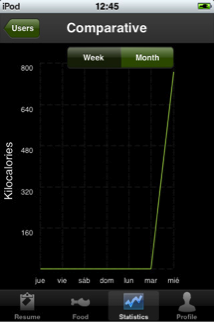
\includegraphics[width=0.5\textwidth]{images/smart-diet-2}
\caption{Smart Diet UI}
\label{fig:smart-diet-2}
\end{figure}

\subsubsection{M-AID}

\paragraph{} An app to support emergency medical treatment\footnote{\url{http://journals.lww.com/ejanaesthesiology/Fulltext/2007/06001/Evaluation_of_M_AID,_a_mobile_phone_first_aid.619.aspx}}

\paragraph{Background and Goal of Study} ``Cardiopulmonary resuscitation (CPR) by bystanders has been shown to reduce mortality due to sudden cardiac arrest when it is effectively performed.'' A mobile app detailing the steps for diagnosis and treatment was developed – called M-AID. The study wanted to see whether it was useful in an emergency situation.
Normally evaluation studies would need to compare against a control group. So if a new drug is developed they need one group to take the placebo to check whether the improvements are real or perceived.
Ethically, you can’t give 100 people the app and 100 people a dummy app and count the lives saved so they designed a scenario-based experiment – or simulated instances of cardiac arrest. The test group had the M-AID app and the control group didn’t have the app.

\paragraph{Materials and Methods} ``119 volunteers were randomly assigned either to the test or the control group. All participants had to manage the same emergency scenario - acute coronary syndrome leading to cardiac arrest. The participants were either equipped with a mobile phone running M-AID (test group) or had to handle the situation without any support (control group).''
The experiment was observed – with points allocated for each correct action taken. The scores were then compared. Some statistical levelling was introduced according to the participant’s medical training and experience. The participant’s mobile phone previous use and expertise was also recorded for the study. 
Results and Discussions: “The test group achieved a slightly higher average score that was not statistically significant (21.11 vs. 19.97; p = 0.302). In contrast, the performance of the individuals in the control group was significantly faster (2.41 min. vs. 4.24min; p < 0.001). Subgroup analysis showed that experienced mobile phone users performed significantly better than non experienced individuals, but not as good as participants with advanced first aid knowledge.”
\paragraph{Conclusions} ``Experience in the use of mobile phones is a precondition for the efficient use of the tested M-AID version. Furthermore, the software cannot replace skills acquisition by practical training. In a subgroup with experience in the handling of mobile phones and basic knowledge in CPR, the device improved performance of CPR.''

\begin{figure}[H]
\centering
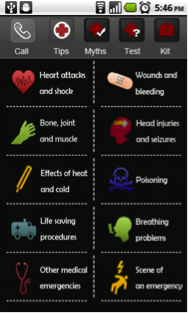
\includegraphics[width=0.5\textwidth]{images/m-aid-1}
\caption{M-AID main screen}
\label{fig:m-aid-1}
\end{figure}

\begin{figure}[H]
\centering
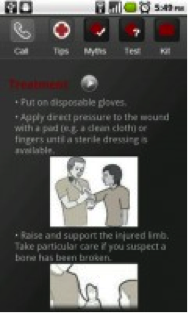
\includegraphics[width=0.5\textwidth]{images/m-aid-2}
\caption{Detail of the M-Aid advice}
\label{fig:m-aid-2}
\end{figure}

\section{Conclusions}
\paragraph{} Evaluation is largely the same as website/ desktop app evaluation but it has to include context. Don’t forget that the usability lab is less effective for mobile app evaluation than when you are evaluating a desktop app or a website. For mobile apps we have to move out to typical locations and situations: for example – inside, outside, in a crowd, in a park, on a bus. Think about both mobility and space. Engineer other interactions such as interruptions with phone and SMS events to see how your user can cope with your application while dealing with other typical events.

\paragraph{} Now your environment or context includes at night as well as during the day, at a rock concert, in a cathedral or in a supermarket. Never forget, however, that evaluation has to be proportionate. If you think you might sell 100 copies of your £0.79 app don’t go mad and pay users and psychologists to design a series of tests.



\section{Summary}
\paragraph{} We have looked at a range of topics related to the design and evaluation of mobile apps. You should now be able to:

\begin{itemize}
\item Use design patterns to communicate your designs
\item Use and understand platform guidelines
\item Evaluate your application
\end{itemize}

%\section{References \& Resources}

